% Gerado automaticamente. No preambulo do documento use:
% \usepackage{pgfplots}
% \pgfplotsset{compat=1.18}
\definecolor{plotblue}{HTML}{2563EB}
\definecolor{plotorange}{HTML}{D97706}
\definecolor{plotgreen}{HTML}{059669}
\definecolor{plotpurple}{HTML}{7C3AED}
\definecolor{plotgray}{HTML}{374151}
\definecolor{plotred}{HTML}{DC2626}
\definecolor{plotteal}{HTML}{0F766E}
\definecolor{plotslate}{HTML}{64748B}

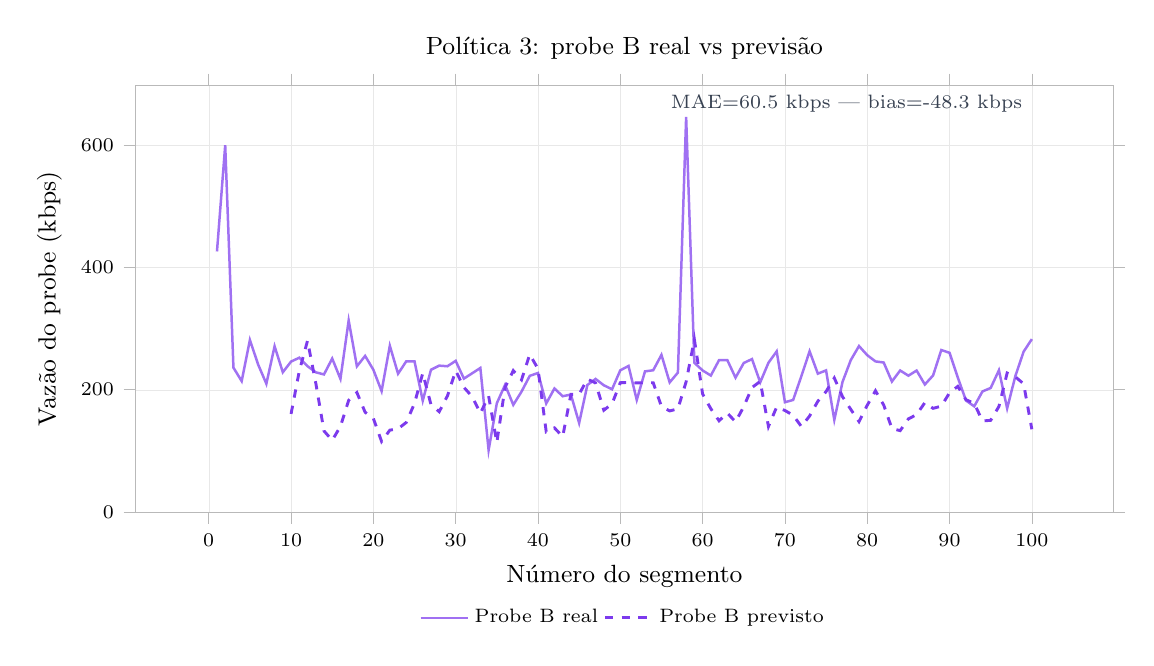
\begin{tikzpicture}
\begin{axis}[
    title={Política 3: probe B real vs previsão},
    xlabel={Número do segmento},
    ylabel={Vazão do probe (kbps)},
    width=14cm,
    height=7cm,
    grid=major,
    grid style={line width=.12pt, draw=gray!18},
    axis line style={draw=gray!55},
    tick style={draw=gray!55},
    tick align=outside,
    title style={font=\small},
    label style={font=\small},
    tick label style={font=\scriptsize},
    legend cell align={left},
    legend style={at={(0.5,-0.20)}, anchor=north, legend columns=2, draw=none, font=\scriptsize},
    ymin=0,
    ymax=697.574
]
\addplot+[plotpurple, line width=0.9pt, mark=none, opacity=0.72] coordinates {
(1,426.092)
(2,599.809)
(3,236.119)
(4,214.138)
(5,281.369)
(6,241.223)
(7,209.76)
(8,271.083)
(9,228.606)
(10,246.035)
(11,252.397)
(12,238.548)
(13,228.536)
(14,225.019)
(15,250.991)
(16,217.739)
(17,313.237)
(18,238.35)
(19,255.301)
(20,232.683)
(21,197.739)
(22,271.89)
(23,226.183)
(24,246.545)
(25,246.351)
(26,182.109)
(27,232.655)
(28,239.388)
(29,238.41)
(30,247.216)
(31,218.17)
(33,235.583)
(34,101.186)
(35,177.927)
(36,207.951)
(37,175.292)
(38,196.936)
(39,222.693)
(40,227.379)
(41,177.593)
(42,202.089)
(43,189.383)
(44,192.122)
(45,145.615)
(46,207.776)
(47,217.655)
(48,207.258)
(49,200.779)
(50,231.788)
(51,238.874)
(52,183.308)
(53,230.005)
(54,231.873)
(55,256.987)
(56,211.996)
(57,228.085)
(58,645.902)
(59,243.999)
(60,231.568)
(61,223.197)
(62,248.443)
(63,248.483)
(64,219.76)
(65,243.739)
(66,250.131)
(67,212.133)
(68,244.076)
(69,262.747)
(70,179.605)
(71,183.295)
(72,222.209)
(73,262.833)
(74,226.28)
(75,231.652)
(76,150.571)
(77,212.845)
(78,248.377)
(79,271.436)
(80,256.548)
(81,246.327)
(82,244.533)
(83,213.422)
(84,231.513)
(85,223.011)
(86,231.366)
(87,208.573)
(88,223.33)
(89,264.928)
(90,260.413)
(91,220.124)
(92,182.339)
(93,172.875)
(94,197.216)
(95,202.911)
(96,231.876)
(97,169.483)
(98,222.489)
(99,262.227)
(100,282.778)
};
\addlegendentry{Probe B real}
\addplot+[plotpurple, dashed, line width=1.05pt, mark=none] coordinates {
(10,160.49)
(11,230.487)
(12,280.09)
(13,211.262)
(14,132.66)
(15,117.309)
(16,140.047)
(17,182.71)
(18,195.354)
(19,163.179)
(20,153.069)
(21,115.399)
(22,133.912)
(23,136.174)
(24,146.556)
(25,177.773)
(26,227.063)
(27,175.692)
(28,164.087)
(29,189.947)
(30,230.971)
(31,203.87)
(32,188.83)
(33,161.481)
(34,189.862)
(35,113.681)
(36,203.95)
(37,231.234)
(38,216.197)
(39,257.789)
(40,234.288)
(41,131.279)
(42,137.623)
(43,123.296)
(44,192.397)
(45,192.685)
(46,217.32)
(47,211.107)
(48,166.518)
(49,177.136)
(50,211.501)
(51,211.926)
(52,211.114)
(53,211.71)
(54,211.408)
(55,172.714)
(56,165.361)
(57,168.841)
(58,213.158)
(59,282.177)
(60,193.119)
(61,168.923)
(62,149.219)
(63,161.977)
(64,147.457)
(65,172.446)
(66,203.578)
(67,213.711)
(68,139.906)
(69,171.851)
(70,166.042)
(71,158.353)
(72,139.873)
(73,157.09)
(74,181.203)
(75,196.983)
(76,219.235)
(77,188.639)
(78,167.905)
(79,147.908)
(80,174.574)
(81,198.309)
(82,175.047)
(83,136.578)
(84,133.125)
(85,152.305)
(86,159.359)
(87,178.911)
(88,169.575)
(89,173.146)
(90,194.969)
(91,205.492)
(92,183.695)
(93,177.705)
(94,148.944)
(95,150.007)
(96,172.668)
(97,227.279)
(98,221.055)
(99,209.704)
(100,135.373)
};
\addlegendentry{Probe B previsto}
\node[anchor=north east, font=\scriptsize, plotgray] at (axis cs:100,697.574) {MAE=60.5 kbps | bias=-48.3 kbps};
\end{axis}
\end{tikzpicture}
